\documentclass{beamer}
\usepackage{tikz,amsmath,hyperref,graphicx,stackrel,animate,tipa}
\usetikzlibrary{positioning,shadows,arrows,shapes,calc}
\newcommand{\ipa}[1]{\textipa{#1}}
\newcommand{\argmax}{\operatornamewithlimits{argmax}}
\newcommand{\argmin}{\operatornamewithlimits{argmin}}
\mode<presentation>{\usetheme{Frankfurt}}
\DeclareMathOperator*{\softmax}{softmax}
\AtBeginSection[]
{
  \begin{frame}<beamer>
    \frametitle{Outline}
    \tableofcontents[currentsection,currentsubsection]
  \end{frame}
}
\title{Lecture 15: Baum-Welch}
\author{Mark Hasegawa-Johnson\\All content~\href{https://creativecommons.org/licenses/by/4.0/}{CC-BY 4.0} unless otherwise specified.}
\date{ECE 417: Multimedia Signal Processing, Fall 2021}  
\begin{document}

% Title
\begin{frame}
  \maketitle
\end{frame}

% Title
\begin{frame}
  \tableofcontents
\end{frame}

%%%%%%%%%%%%%%%%%%%%%%%%%%%%%%%%%%%%%%%%%%%%
\section[Review]{Review: Hidden Markov Models}
\setcounter{subsection}{1}

\begin{frame}
  \frametitle{Hidden Markov Model}

  \begin{center}
    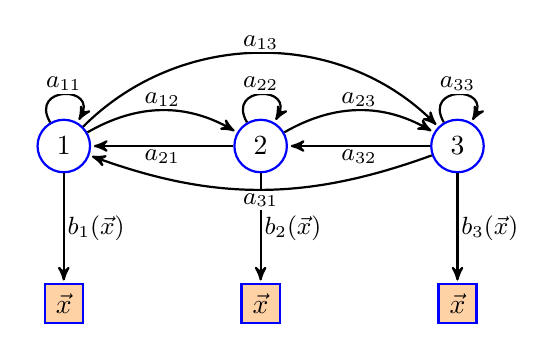
\begin{tikzpicture}[->,>=stealth',shorten >=1pt,auto,node distance=3cm,thick,
        state/.style={circle,thick,draw=blue,text=black,text centered,text width=0.25cm},
        obs/.style={rectangle,thick,draw=blue,text=black,fill=orange!35!white,text centered,text width=0.25cm}
      ]
      \node[state] (q1) at (0,0) {1};
      \node[state] (q2) at (2.5,0) {2};
      \node[state] (q3) at (5,0) {3};
      \node[obs] (x1) at (0,-2) {$\vec{x}$};
      \node[obs] (x2) at (2.5,-2) {$\vec{x}$};
      \node[obs] (x3) at (5,-2) {$\vec{x}$};
      \path[every node/.style={font=\sffamily\small,
  	  fill=white,inner sep=1pt}]
      (q1) edge [out=120,in=60,looseness=4] node {$a_{11}$} (q1)
      edge [out=30,in=150] node {$a_{12}$} (q2)
      edge [out=45,in=135] node {$a_{13}$} (q3)
      edge [out=-90,in=90] node {$b_1(\vec{x})$} (x1)
      (q2) edge [out=120,in=60,looseness=4] node {$a_{22}$} (q2)
      edge [out=180,in=0] node {$a_{21}$} (q1)
      edge [out=30,in=150] node {$a_{23}$} (q3)
      edge [out=-90,in=90] node {$b_2(\vec{x})$} (x2)
      (q3) edge [out=120,in=60,looseness=4] node {$a_{33}$} (q3)
      edge [out=180,in=0] node {$a_{32}$} (q2)
      edge [out=-160,in=-20] node {$a_{31}$} (q1)
      edge [out=-90,in=90] node {$b_3(\vec{x})$} (x3);
    \end{tikzpicture}
  \end{center}
  \begin{enumerate}
  \item Start in state $q_t=i$ with pmf $\pi_i$.
  \item Generate an observation, $\vec{x}$, with pdf $b_i(\vec{x})$.
  \item Transition to a new state, $q_{t+1}=j$, according to pmf $a_{ij}$.
  \item Repeat.
  \end{enumerate}
\end{frame}


\begin{frame}
  \frametitle{The Three Problems for an HMM}

  \begin{enumerate}
  \item {\bf Recognition:} Given two different HMMs, $\Lambda_1$ and
    $\Lambda_2$, and an observation sequence $X$.  Which HMM was more
    likely to have produced $X$?  In other words, 
    $p(X|\Lambda_1)>p(X|\Lambda_2)$?
  \item {\bf Segmentation:} What is $p(q_t=i|X,\Lambda)$?
  \item {\bf Training:} Given an initial HMM $\Lambda$, and an
    observation sequence $X$, can we find $\Lambda'$ such that
    $p(X|\Lambda') > p(X|\Lambda)$?
  \end{enumerate}
\end{frame}

\begin{frame}
  \frametitle{The Forward Algorithm}

  Definition: $\alpha_t(i) \equiv p(\vec{x}_1,\ldots,\vec{x}_t,q_t=i|\Lambda)$.  Computation:
  \begin{enumerate}
  \item {\bf Initialize:}
    \[
    \alpha_1(i) = \pi_i b_i(\vec{x}_1),~~~1\le i\le N
    \]
  \item {\bf Iterate:}
    \begin{align*}
      \alpha_{t}(j) &= \sum_{i=1}^N \alpha_{t-1}(i) a_{ij}b_j(\vec{x}_t),~~1\le j\le N,~2\le t\le T
    \end{align*}
  \item {\bf Terminate:}
    \[
    p(X|\Lambda) = \sum_{i=1}^N \alpha_T(i)
    \]
  \end{enumerate}
\end{frame}
  
\begin{frame}
  \frametitle{The Backward Algorithm}

  Definition: $\beta_t(i) \equiv p(\vec{x}_{t+1},\ldots,\vec{x}_T|q_t=i,\Lambda)$.  Computation:
  \begin{enumerate}
  \item {\bf Initialize:}
    \[
    \beta_T(i) = 1,~~~1\le i\le N
    \]
  \item {\bf Iterate:}
    \begin{align*}
      \beta_{t}(i) &= \sum_{j=1}^N a_{ij}b_j(\vec{x}_{t+1})\beta_{t+1}(j),~~1\le i\le N,~1\le t\le T-1
    \end{align*}
  \item {\bf Terminate:}
    \[
    p(X|\Lambda) = \sum_{i=1}^N \pi_ib_i(\vec{x}_1)\beta_1(i)
    \]
  \end{enumerate}
\end{frame}

\begin{frame}
  \frametitle{Segmentation}

  \begin{enumerate}
  \item {\bf The State Posterior:}
    \begin{align*}
      \gamma_t(i) & = p(q_t=i|X,\Lambda)
      = \frac{\alpha_t(i)\beta_t(i)}{\sum_{k=1}^N\alpha_t(k)\beta_t(k)}
    \end{align*}
  \item {\bf The Segment Posterior:}
    \begin{align*}
      \xi_t(i,j) & = p(q_t=i,q_{t+1}=j|X,\Lambda)\\
      &= \frac{\alpha_t(i)a_{ij}b_j(\vec{x}_{t+1})\beta_{t+1}(j)}{\sum_{k=1}^N\sum_{\ell=1}^N\alpha_t(k)a_{k\ell}b_\ell(\vec{x}_{t+1})\beta_{t+1}(\ell)}
    \end{align*}
  \end{enumerate}
\end{frame}


\begin{frame}
  \frametitle{The Three Problems for an HMM}

  \begin{enumerate}
  \item {\bf Recognition:} Given two different HMMs, $\Lambda_1$ and
    $\Lambda_2$, and an observation sequence $X$.  Which HMM was more
    likely to have produced $X$?  In other words, 
    $p(X|\Lambda_1)>p(X|\Lambda_2)$?
  \item {\bf Segmentation:} What is $p(q_t=i|X,\Lambda)$?
  \item {\bf Training:} Given an initial HMM $\Lambda$, and an
    observation sequence $X$, can we find $\Lambda'$ such that
    $p(X|\Lambda') > p(X|\Lambda)$?
  \end{enumerate}
\end{frame}


%%%%%%%%%%%%%%%%%%%%%%%%%%%%%%%%%%%%%%%%%%%%
\section[ML]{Maximum-Likelihood  Training of an HMM}
\setcounter{subsection}{1}

\begin{frame}
  \frametitle{Maximum Likelihood Training}
  
  Suppose we're given several observation sequences of the form
  $X=[\vec{x}_1,\ldots,\vec{x}_T]$.  Suppose, also, that we have some
  initial guess about the values of the model parameters (our initial
  guess doesn't have to be very good).  Maximum likelihood training
  means we want to compute a new set of parameters,
  $\Lambda'=\left\{\pi_i',a_{ij}',b_j'(\vec{x})\right\}$ that maximize
  $p(X|\Lambda')$.
  \begin{enumerate}
  \item {\bf Initial State Probabilities:} Find values of $\pi_i'$, $1\le
    i\le N$, that maximize $p(X|\Lambda')$.
  \item {\bf Transition Probabilities:} Find values of $a_{ij}'$, $1\le
    i,j\le N$, that maximize $p(X|\Lambda')$.
  \item {\bf Observation Probabilities:} Learn $b_j'(\vec{x})$.  What does that
    mean, actually?
  \end{enumerate}
\end{frame}

\begin{frame}
  \frametitle{Learning the Observation Probabilities}

  There are four typical ways of learning the observation probabilities, $b_j(\vec{x})$.
    \begin{enumerate}
    \item Vector quantize $\vec{x}$, using some VQ method.  Suppose
      $\vec{x}$ is the $k^{\textrm{th}}$ codevector; then we just need
      to learn $b_j(k)$ such that
      \[
      b_j(j)\ge 0,~~~\sum_{k=0}^{K-1} b_j(k)=1
      \]
    \item Model $b_j(k)$ as a Gaussian or mixture Gaussian, and learn
      its parameters.
    \item Model $b_j(k)$ as a  neural net, and learn its parameters.
    \end{enumerate}
\end{frame}
  
\begin{frame}
  \frametitle{Maximum Likelihood Training}
  
  For now, suppose that we have the following parameters that we need to learn:
  \begin{enumerate}
  \item {\bf Initial State Probabilities:} $\pi_i'$ such that
    \[
    \pi_i' \ge 0,~~~\sum_{i=1}^N \pi_i' = 1
    \]
  \item {\bf Transition Probabilities:} $a_{ij}'$ such that
    \[
    a_{ij}'\ge 0,~~~\sum_{j=1}^N a_{ij}' =1
    \]
  \item {\bf Observation Probabilities:} $b_j'(k)$ such that
    \[
    b_j'(k)\ge 0,~~~\sum_{k=1}^{K} b_j'(k)=1
    \]
  \end{enumerate}
\end{frame}

\begin{frame}
  \frametitle{Maximum Likelihood Training with Known State Sequence}

  {\bf Impossible assumption}: Suppose that we actually know the state
  sequences, $Q=[q_1,\ldots,q_T]$, matching with each observation
  sequence $X=[\vec{x}_1,\ldots,\vec{x}_T]$.  Then what would be the
  maximum-likelihood parameters?

\end{frame}

\begin{frame}
  \frametitle{Maximum Likelihood Training with Known State Sequence}

  Our goal is to find $\Lambda=\left\{\pi_i,a_{ij},b_j(k)\right\}$ in
  order to maximize

  \begin{align*}
    {\mathcal L}(\Lambda) &= \ln p(Q,X|\Lambda)\\
    &= \ln \pi_{q_1} + \ln b_{q_1}(x_1) + \ln a_{q_1,q_2} + b_{q_2}(x_2) + \ldots\\
    &= \ln\pi_{q_1} + \sum_{i=1}^N\left(\sum_{j=1}^N n_{ij}\ln a_{ij} + \sum_{k=1}^Km_{ik}\ln b_i(k)\right)
  \end{align*}
  where
  \begin{itemize}
  \item $n_{ij}$ is the number of times we saw $(q_{t}=i,q_{t+1}=j)$,
  \item $m_{ik}$ is the number of times we saw $(q_t=i,k_t=k)$
  \end{itemize}
\end{frame}

\begin{frame}
  \frametitle{Maximum Likelihood Training with Known State Sequence}

  \begin{align*}
    {\mathcal L}(\Lambda) 
    &= \ln\pi_{q_1} + \sum_{i=1}^N\left(\sum_{j=1}^N n_{ij}\ln a_{ij} + \sum_{k=1}^Km_{ik}\ln b_i(k)\right)
  \end{align*}
  When we differentiate that, we find the following derivatives:
  \begin{align*}
    \frac{\partial\mathcal L}{\partial \pi_i} &= \begin{cases}
      \frac{1}{\pi_i}& i=q_1\\0& \mbox{otherwise}\end{cases}\\
    \frac{\partial\mathcal L}{\partial a_{ij}} &= \frac{n_{ij}}{a_{ij}}\\
    \frac{\partial\mathcal L}{\partial b_j(k)} &= \frac{m_{jk}}{b_{j}(k)}
  \end{align*}
  These derivatives are {\bf never} equal to zero!  What went wrong?
\end{frame}

\begin{frame}
  \frametitle{Maximum Likelihood Training with Known State Sequence}

  Here's the problem: we forgot to include the constraints
  $\sum_i\pi_i=1$, $\sum_j a_{ij}=1$, and $\sum_k b_j(k)=1$!

  We can include the constraints using the method of Lagrange multipliers.  If we do that,
  we wind up with the solutions
  \begin{align*}
    \pi_i' &= \begin{cases}\frac{1}{\lambda} & i=q_1\\0&\mbox{otherwise}\end{cases}\\
    a_{ij}' &= \frac{n_{ij}}{\mu_i}\\
    b_j(k)' &= \frac{m_{jk}}{\nu_j}
  \end{align*}
  where $\lambda$, $\mu_i$, and $\nu_j$ are {\bf arbitrary constants}
  (called Lagrange multipliers) that we can set to any value we want,
  provided that the constraints are satisfied.
\end{frame}

\begin{frame}
  \frametitle{Maximum Likelihood Training with Known State Sequence}

  Using the Lagrange multiplier method, we can show that the maximum likelihood  parameters
  for the HMM are:
  \begin{enumerate}
  \item {\bf Initial State Probabilities:}
    \[
    \pi_i'=\frac{\mbox{\# state sequences that start with}~q_1=i}{\mbox{\# state sequences in training data}}
    \]
  \item {\bf Transition Probabilities:}
    \[
    a_{ij}'=\frac{\mbox{\# frames in which}~q_{t-1}=i,q_t=j}{\mbox{\# frames in which}~q_{t-1}=i}
    \]
  \item {\bf Observation Probabilities:} 
    \[
    b_j'(k)=\frac{\mbox{\# frames in which}~q_t=j,k_t=k}{\mbox{\# frames in which}~q_{t}=j}
    \]
  \end{enumerate}
\end{frame}

  
%%%%%%%%%%%%%%%%%%%%%%%%%%%%%%%%%%%%%%%%%%%%
\section[Baum-Welch]{Baum-Welch: the EM Algorithm for Markov Models}
\setcounter{subsection}{1}

\begin{frame}
  \frametitle{Expectation Maximization}

  When the true state sequence is unknown, then we can't maximize the
  likelihood $p(X,Q|\Lambda')$ directly.  Instead, we maximize the {\em
    expected} log likelihood.  This is an instance of the EM algorithm, where
  the visible training dataset is
  \begin{displaymath}
    {\mathcal D}_v = \left\{\vec{x}_1,\ldots,\vec{x}_T\right\}
  \end{displaymath}
  and the hidden dataset is
  \begin{displaymath}
    {\mathcal D}_h = \left\{q_1,\ldots,q_T\right\}
  \end{displaymath}
\end{frame}

\begin{frame}
  \frametitle{Expectation Maximization: the M-Step}

  In the M-step of EM, we use the E-step probabilities to calculate
  the {\bf expected} maximum likelihood estimators:
  \begin{enumerate}
  \item {\bf Initial State Probabilities:}
    \[
    \pi_i'=\frac{E\left[\mbox{\# state sequences that start with}~q_1=i\right]}{\mbox{\# state sequences in training data}}
    \]
  \item {\bf Transition Probabilities:}
    \[
    \pi_i'=\frac{E\left[\mbox{\# frames in which}~q_{t-1}=i,q_t=j\right]}{E\left[\mbox{\# frames in which}~q_{t-1}=i\right]}
    \]
  \item {\bf Observation Probabilities:} 
    \[
    b_j'(k)=\frac{E\left[\mbox{\# frames in which}~q_t=j,k_t=k\right]}{E\left[\mbox{\# frames in which}~q_{t}=j\right]}
    \]
  \end{enumerate}
\end{frame}


\begin{frame}
  \frametitle{Expectation Maximization: the E-Step}

  In order to find quantities like ``the expected number of times $q_1=i$,'' we need to
  do the E-Step of EM.  The E-step calculates probabilities like:
  \begin{align*}
    p({\mathcal D}_h|{\mathcal D}_v,\Lambda)
  \end{align*}
  For example, in order to re-estimate $b_j(k)$, we need to know the
  \# frames in which $q_t=i$. For that, we need
  \begin{align*}
    p(q_t=i|\vec{x}_1,\vec{x}_2,\ldots,\vec{x}_T,\Lambda)
  \end{align*}
  \ldots but this is something we already know!  It is
  \begin{align*}
    p(q_t=i|\vec{x}_1,\vec{x}_2,\ldots,\vec{x}_T,\Lambda) = \gamma_t(i)
  \end{align*}  
\end{frame}

\begin{frame}
  \frametitle{Expectation Maximization: the E-Step}

  Similarly, in order to re-estimate $a_{ij}$, we need to know the
  \# frames in which $q_{t-1}=i$ and $q_t=j$. For that, we need
  $p(q_{t-1}=i,q_t=j|\vec{x}_1,\vec{x}_2,\ldots,\vec{x}_T,\Lambda)$:
  \begin{itemize}
  \item In the $t^{\textrm{th}}$ frame, the event $q_{t}=i,q_{t+1}=j$ either
    happens, or it doesn't happen.
  \item So the following  expectation is actually just a  probability:
    \begin{align*}
      & E\left[\mbox{\# times during the $t^{\textrm{th}}$ frame, in which}~q_{t}=i,q_{t+1}=j\right] \\
      & = p(q_{t}=i,q_{t+1}=j)\\
      &= \xi_t(i,j)
    \end{align*}
  \end{itemize}
\end{frame}


\begin{frame}
  \frametitle{The Baum-Welch Algorithm}

  \begin{enumerate}
  \item {\bf Initial State Probabilities:}
    \begin{align*}
      \pi_i'&=\frac{E\left[\mbox{\# state sequences that start with}~q_1=i\right]}{\mbox{\# state sequences in training data}}\\
      &=\frac{\sum_{sequences} \gamma_1(i)}{\mbox{\# sequences}}
    \end{align*}
  \end{enumerate}
\end{frame}

\begin{frame}
  \frametitle{The Baum-Welch Algorithm}

  \begin{enumerate}
  \item {\bf Initial State Probabilities:}
    \begin{align*}
      \pi_i'  &=\frac{\sum_{sequences} \gamma_1(i)}{\mbox{\# sequences}}
    \end{align*}
  \item {\bf Transition Probabilities:}
    \begin{align*}
      a_{ij}'&=\frac{E\left[\mbox{\# frames in which}~q_{t-1}=i,q_t=j\right]}{E\left[\mbox{\# frames in which}~q_{t-1}=i\right]}\\
      &=\frac{\sum_{t=1}^{T-1} \xi_t(i,j)}{\sum_{j=1}^N\sum_{t=1}^{T-1}\xi_t(i,j)}
    \end{align*}
  \end{enumerate}
\end{frame}

\begin{frame}
  \frametitle{The Baum-Welch Algorithm}

  \begin{enumerate}
  \item {\bf Initial State Probabilities:}
    \begin{align*}
      \pi_i' &=\frac{\sum_{sequences} \gamma_1(i)}{\mbox{\# sequences}}
    \end{align*}
  \item {\bf Transition Probabilities:}
    \begin{align*}
      a_{ij}' &=\frac{\sum_{t=1}^{T-1} \xi_t(i,j)}{\sum_{j=1}^N\sum_{t=1}^{T-1}\xi_t(i,j)}
    \end{align*}
  \item {\bf Observation Probabilities:} 
    \begin{align*}
      b_{j}'(k) &=\frac{E\left[\mbox{\# frames in which}~q_{t}=j,k_t=k\right]}{E\left[\mbox{\# frames in which}~q_{t}=j\right]}
    \end{align*}
  \end{enumerate}
\end{frame}

\begin{frame}
  \frametitle{The Baum-Welch Algorithm}

  \begin{enumerate}
  \item {\bf Initial State Probabilities:}
    \begin{align*}
      \pi_i' &=\frac{\sum_{sequences} \gamma_1(i)}{\mbox{\# sequences}}
    \end{align*}
  \item {\bf Transition Probabilities:}
    \begin{align*}
      a_{ij}' &=\frac{\sum_{t=1}^{T-1} \xi_t(i,j)}{\sum_{j=1}^N\sum_{t=1}^{T-1}\xi_t(i,j)}
    \end{align*}
  \item {\bf Observation Probabilities:} 
    \begin{align*}
      b_{j}'(k) 
      &=\frac{\sum_{t:\vec{x}_t=k} \gamma_t(j)}{\sum_{t}\gamma_t(j)}
    \end{align*}
  \end{enumerate}
\end{frame}


%%%%%%%%%%%%%%%%%%%%%%%%%%%%%%%%%%%%%%%%%%%%
\section[Gaussians]{Gaussian Observation Probabilities}
\setcounter{subsection}{1}

\begin{frame}
  \frametitle{Baum-Welch with Gaussian Probabilities}

  The requirement that we vector-quantize the observations is a
  problem.  It means that we can't model the observations very precisely.

  It would be better if we could model the observation likelihood,
  $b_j(\vec{x})$, as a probability density in the space
  $\vec{x}\in\Re^D$.  One way is to use a parameterized function that
  is guaranteed to be a properly normalized pdf.  For example, a
  Gaussian:
  \begin{displaymath}
    b_i(\vec{x}) = {\mathcal N}\left(\vec{x};\vec\mu_i,\Sigma_i\right)
  \end{displaymath}
\end{frame}
  
\begin{frame}
  \frametitle{Diagonal-Covariance Gaussian pdf}

  Let's assume the feature vector has $D$ dimensions,
  $\vec{x}_t=[x_{t,1},\ldots,x_{t,D}]$.  The Gaussian pdf is
  \begin{displaymath}
    b_i(\vec{x}_t) = 
    \frac{1}{(2\pi)^{D/2}|\Sigma_i|^{1/2}}e^{-\frac{1}{2}(\vec{x}_t-\vec\mu_i)\Sigma_i^{-1}(\vec{x}_t-\vec\mu_i)^T}
  \end{displaymath}
  The logarithm of a Gaussian is
  \begin{displaymath}
    \ln b_i(\vec{x}_t)=
    -\frac{1}{2}\left((\vec{x}_t-\vec\mu_i)^T\Sigma_i^{-1}(\vec{x}_t-\vec\mu_i)
    +\ln|\Sigma_i| + C\right)
  \end{displaymath}
  where the constant is $C=D\ln(2\pi)$.
\end{frame}

\begin{frame}
  \frametitle{Expectation maximization}

  Expectation maximization maximizes the expected
  log probability, i.e.,
  \begin{displaymath}
    E\left[\ln b_i(\vec{x}_t)\right]=
    -\frac{1}{2}\sum_{i=1}^N \gamma_t(i)\left(
    (\vec{x}_t-\vec\mu_i)^T\Sigma_i^{-1}(\vec{x}_t-\vec\mu_i)
    +\ln|\Sigma_i|+C\right)
  \end{displaymath}
  If we include all of the frames, then we get
  \begin{align*}
    E\left[\ln p(X,Q|\Lambda)\right] &= \mbox{other terms}\\
    &-\frac{1}{2}\sum_{t=1}^T \sum_{i=1}^N \gamma_t(i)\left(
    (\vec{x}_t-\vec\mu_i)^T\Sigma_i^{-1}(\vec{x}_t-\vec\mu_i)
    +\ln|\Sigma_i|+C\right) 
  \end{align*}
  where the ``other terms'' are about $a_{ij}$ and $\pi_i$, and have
  nothing to do with $\vec\mu_i$ or $\Sigma_i$.
\end{frame}
  
\begin{frame}
  \frametitle{M-Step: optimum $\vec\mu$}

  First, let's optimize $\vec\mu$.  We want
  \begin{displaymath}
    0 = \nabla_{\vec\mu_q}\sum_{t=1}^T\sum_{i=1}^N\gamma_t(i)(\vec{x}_t-\vec\mu_i)^T\Sigma_i^{-1}(\vec{x}_t-\vec\mu_i)
  \end{displaymath}
  Re-arranging terms, we get
  \begin{displaymath}
    \vec\mu_q' = \frac{\sum_{t=1}^T\gamma_t(q)\vec{x}_{t}}{\sum_{t=1}^T\gamma_t(q)}
  \end{displaymath}
\end{frame}

\begin{frame}
  \frametitle{M-Step: optimum $\Sigma$}

  Second, let's optimize $\Sigma_{i}$.  In order to do this, we need
  to talk about the gradient of a scalar w.r.t. a matrix.  Let's
  suppose that
  \begin{displaymath}
    \Sigma = \left[\begin{array}{ccc}
        \sigma_1^2 & \cdots & \rho_{1,D}\\
        \vdots & \ddots & \vdots\\
        \rho_{D,1} & \cdots & \sigma_D^2
      \end{array}
      \right]
  \end{displaymath}
  When we talk about $\nabla_\Sigma f(\Sigma)$, for some scalar
  function $f(\cdot)$, what we mean is the matrix whose elements are 
  \begin{displaymath}
    \nabla_\Sigma f(\Sigma) = \left[\begin{array}{ccc}
        \frac{\partial f}{\partial\sigma_1^2} & \cdots & \frac{\partial f}{\partial\rho_{1,D}}\\
        \vdots & \ddots & \vdots\\
        \frac{\partial f}{\partial\rho_{D,1}} & \cdots & \frac{\partial f}{\partial\sigma_D^2}
      \end{array}
      \right]
  \end{displaymath}
\end{frame}

\begin{frame}
  \frametitle{M-Step: optimum $\Sigma$}

  In particular, for a positive-definite, symmetric $\Sigma$, it's possible to show that
  \begin{displaymath}
    \nabla_\Sigma \ln|\Sigma| = \Sigma^{-1}
  \end{displaymath}
  and
  \begin{displaymath}
    \nabla_\Sigma (\vec{x}-\vec\mu)^T\Sigma^{-1}(\vec{x}-\vec\mu) = -\Sigma^{-1}(\vec{x}-\vec\mu)(\vec{x}-\vec\mu)^T\Sigma^{-1}
  \end{displaymath}
\end{frame}
  
  
\begin{frame}
  \frametitle{Minimizing the cross-entropy: optimum $\sigma$}

  Taking advantage of those facts, let's find
  \begin{displaymath}
    0 = \nabla_{\Sigma_q}\sum_{t=1}^T\sum_{i=1}^N\gamma_t(i)\left(\ln|\Sigma_i|+
    (\vec{x}_{t}-\vec\mu_{i})^T\Sigma_i^{-1}(\vec{x}_t-\vec\mu_i)\right)
  \end{displaymath}
  Re-arranging terms, we get
  \begin{displaymath}
    \Sigma_{q}' = \frac{\sum_{t=1}^T\gamma_t(q)(\vec{x}_{t}-\vec\mu_{q})(\vec{x}_t-\vec\mu_q)^T}{\sum_{t=1}^T\gamma_t(q)}
  \end{displaymath}
\end{frame}

\begin{frame}
  \frametitle{Summary: Gaussian Observation PDFs}

  So we can use Gaussians for $b_j(\vec{x})$:
  \begin{itemize}
  \item {\bf E-Step:}
    \[
    \gamma_t(i) = \frac{\alpha_t(i)\beta_t(i)}{\sum_{i'}\alpha_t(i')\beta_t(i')}
    \]
  \item {\bf M-Step:}
    \begin{displaymath}
      \vec\mu_{i}' = \frac{\sum_{t=1}^T\gamma_t(i)\vec{x}_{t}}{\sum_{t=1}^T\gamma_t(i)}
    \end{displaymath}
    \begin{displaymath}
      \Sigma_{i}' = \frac{\sum_{t=1}^T\gamma_t(i)(\vec{x}_{t}-\vec\mu_{i})(\vec{x}_t-\vec\mu_i)^T}{\sum_{t=1}^T\gamma_t(i)}
    \end{displaymath}
  \end{itemize}
\end{frame}


%%%%%%%%%%%%%%%%%%%%%%%%%%%%%%%%%%%%%%%%%%%%
\section[Summary]{Summary}
\setcounter{subsection}{1}

\begin{frame}
  \frametitle{The Baum-Welch Algorithm: Initial and Transition Probabilities}

  \begin{enumerate}
  \item {\bf Initial State Probabilities:}
    \begin{align*}
      \pi_i' &=\frac{\sum_{sequences} \gamma_1(i)}{\mbox{\# sequences}}
    \end{align*}
  \item {\bf Transition Probabilities:}
    \begin{align*}
      a_{ij}' &=\frac{\sum_{t=1}^{T-1} \xi_t(i,j)}{\sum_{j=1}^N\sum_{t=1}^{T-1}\xi_t(i,j)}
    \end{align*}
  \end{enumerate}
\end{frame}

\begin{frame}
  \frametitle{The Baum-Welch Algorithm: Observation Probabilities}
  \begin{enumerate}
  \item {\bf Discrete Observation Probabilities:}
    \begin{align*}
      b_{j}'(k) &=\frac{\sum_{t:\vec{x}_t=k} \gamma_t(j)}{\sum_{t}\gamma_t(j)}
    \end{align*}
  \item {\bf Gaussian Observation PDFs:}
    \begin{displaymath}
      \vec\mu_{i}' = \frac{\sum_{t=1}^T\gamma_t(i)\vec{x}_{t}}{\sum_{t=1}^T\gamma_t(i)}
    \end{displaymath}
    \begin{displaymath}
      \Sigma_{i}' = \frac{\sum_{t=1}^T\gamma_t(i)(\vec{x}_{t}-\vec\mu_{i})(\vec{x}_t-\vec\mu_i)^T}{\sum_{t=1}^T\gamma_t(i)}
    \end{displaymath}
  \end{enumerate}
\end{frame}

%%%%%%%%%%%%%%%%%%%%%%%%%%%%%%%%%%%%%%%%%%%%
\section[Example]{Written Example}
\setcounter{subsection}{1}

\begin{frame}
  \frametitle{Written Example}

  In a second-order Markov process, $q_t$ depends on both $q_{t-2}$ and
  $q_{t-1}$, thus the model parameters are:
  \begin{align}
    \pi_{ij} &= p(q_1=i,q_2=j)\label{example:pi}\\
    a_{ijk} &= p(q_t=k|q_{t-2}=i,q_{t-1}=i)\\
    b_k(\vec{x}) &= p(\vec{x}|q_t=k)
  \end{align}
  Suppose you have a sequence of observations for which you have
  already $\alpha_t(i,j)$ and $\beta_t(i,j)$, defined as
  \begin{align}
    \alpha_t(i,j) &= p(\vec{x}_1,\ldots,\vec{x}_t,q_{t-1}=i,q_t=j|\Lambda)\\
    \beta_t(i,j) &= p(\vec{x}_{t+1},\ldots,\vec{x}_T|q_{t-1}=i,q_t=j,\Lambda)\label{example:beta}
  \end{align}
  In terms of the quantities defined in Eqs. (\ref{example:pi})
  through (\ref{example:beta}), find a formula that re-estimates
  $a_{ijk}'$ so that, unless $a_{ijk}$ is already optimal, 
  \[
  p(X|\pi_i,a_{ijk}',b_j(\vec{x})) > p(X|\pi_i,a_{ijk},b_j(\vec{x}))
  \]
\end{frame}

\end{document}

